\documentclass{article}
\usepackage{listings}
\usepackage{mathrsfs}
\usepackage[utf8]{inputenc}
\usepackage{amssymb}
\usepackage{lipsum}
\usepackage{amsmath}
\usepackage{fancyhdr}
\usepackage{geometry}
\usepackage{scrextend}
\usepackage[english,german]{babel}
\usepackage{titling}
\setlength{\droptitle}{-3cm}
\usepackage{tikz}
\usepackage{algorithm,algpseudocode}
\usepackage[doublespacing]{setspace}
\usetikzlibrary{datavisualization}
\usetikzlibrary{datavisualization.formats.functions}
\usepackage{polynom}
\usepackage{amsmath}
\usepackage{gauss}
\usepackage{tkz-euclide}
\usetikzlibrary{datavisualization}
\usetikzlibrary{datavisualization.formats.functions}
\author{
Alexander Mattick Kennung: qi69dube\\
Kapitel 1
}
\usepackage{import}
\date{\today}
\geometry{a4paper, margin=2cm}
\usepackage{stackengine}
\parskip 1em
\newcommand\stackequal[2]{%
  \mathrel{\stackunder[2pt]{\stackon[4pt]{=}{$\scriptscriptstyle#1$}}{%
  $\scriptscriptstyle#2$}}
 }
\makeatletter
\renewcommand*\env@matrix[1][*\c@MaxMatrixCols c]{%
  \hskip -\arraycolsep
  \let\@ifnextchar\new@ifnextchar
  \array{#1}}
\makeatother
\lstset{
  language=haskell,
}
\lstnewenvironment{code}{\lstset{language=Haskell,basicstyle=\small}}{}
\usepackage{enumitem}
\setlist{nosep}
\usepackage{titlesec}
\usepackage{ stmaryrd }
\usepackage{verbatim}


\titlespacing*{\subsection}{0pt}{2pt}{3pt}
\titlespacing*{\section}{0pt}{0pt}{5pt}
\titlespacing*{\subsubsection}{0pt}{1pt}{2pt}
\title{Vorlesung 4}


\begin{document}
	\maketitle
	Seien X,Y ZV mit Dichte $f^{(X,Y)}$\\
	$f^{X}(x)=\int_\mathbb{R} f^{(X,Y)}(x,y)dy$\\
	Von vorteil: wenn supp $f^{(X,Y)}$ y-projezierbar ist, dann gilt.\\
	$f^{X}(x)=\int_{\underline{y}}^{\overline{y}} f^{(X,Y)} (x,y) dy$\\
	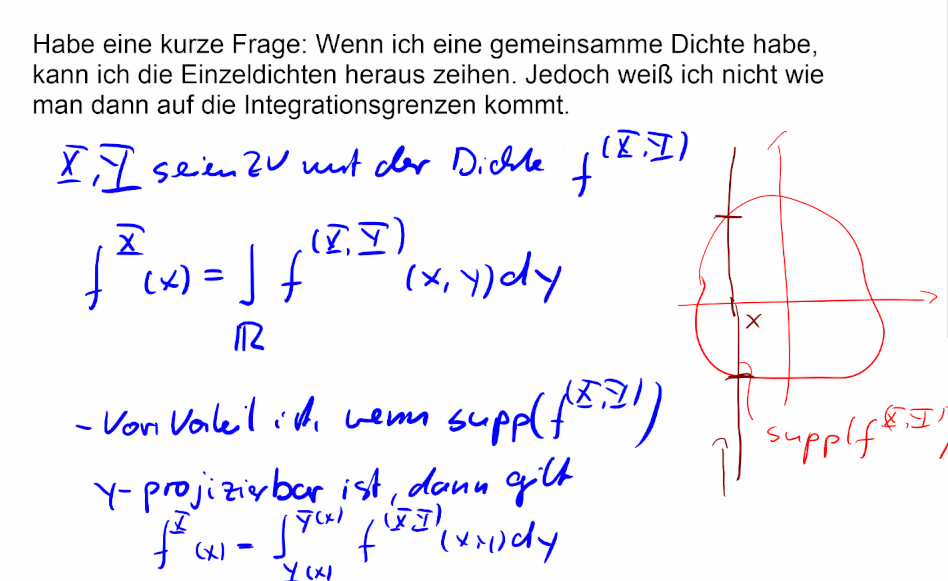
\includegraphics[width=256px]{teildichte.png}\\
	1. $T_N:\Omega_T=\{1,2,3,4\}$ $\mathcal{A} = P(\Omega_T)$\\
	$T_N\sim L(4)$\\
	$P(T_n=t) =\frac{1}{4}$\\
	$Z=\sum ^{T_N} _{i=1} X_i$\\
	somit ist $(t_n,x_1,x_2,x_3,x_4) = (3,6,5,4,6)$\\
	$\sum^3_{i=1} x_i = 6+5+4=15$ (das letze wäre das $X_4$ was nicht mehr drin ist)\\
	der Erwartungswert ist der EW der Zufälligen summe\\
	\includegraphics[width=256px]{Zufällige SUmme.png}\\
	$EZ = ET_N EX = \frac{1+4}{2}\cdot \frac{1+6}{2} = \frac{5+7}{4}$\\
	$Var Z = ET_N\cdot \underbrace{Var X_1}_{identisch\ verteilt}+Var(T_N)\cdot (EX_1)^2=\frac{5}{2}(\frac{6^2-1}{12})+\frac{4^2-1}{12}(\frac{7}{2})^2 = \frac{1085}{48}$.\\
	\[P((X\in B)\cap (Y=y)) = P(X\in B|Y=y)P(Y=y)\]
	\[Var(X)=b,Var(\frac{1}{b}X-a)=Var(\frac{1}{b}X)=\frac{1}{b}\]
	\[T=\frac{1}{\sqrt{b}}X, Var(X)=b\implies Var(T)=1\]
	standardisierung.\\
	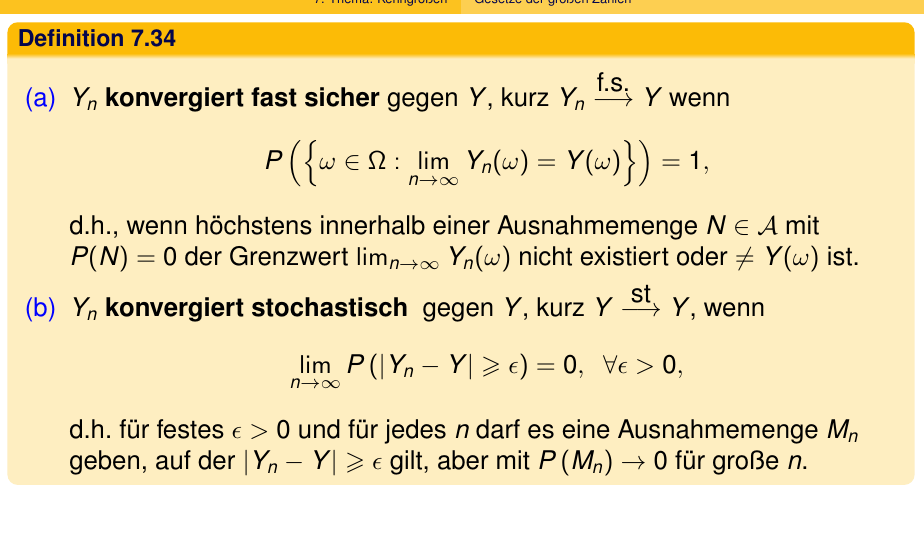
\includegraphics[width=256px]{FastSicher.png}
	konvergiert fast sicher heist, dass der Limes der Reihe gegen eins geht. (Die wahrscheinlichkeit der Ausnahmemenge geht gegen null)\\
	konvergiert stochastisch, dann wird die Differenz zweier Verteilungen Null. (Die wahrscheinlichkeit der Ausnahmemenge wird für ein groß genuges n beliebig klein)\\
	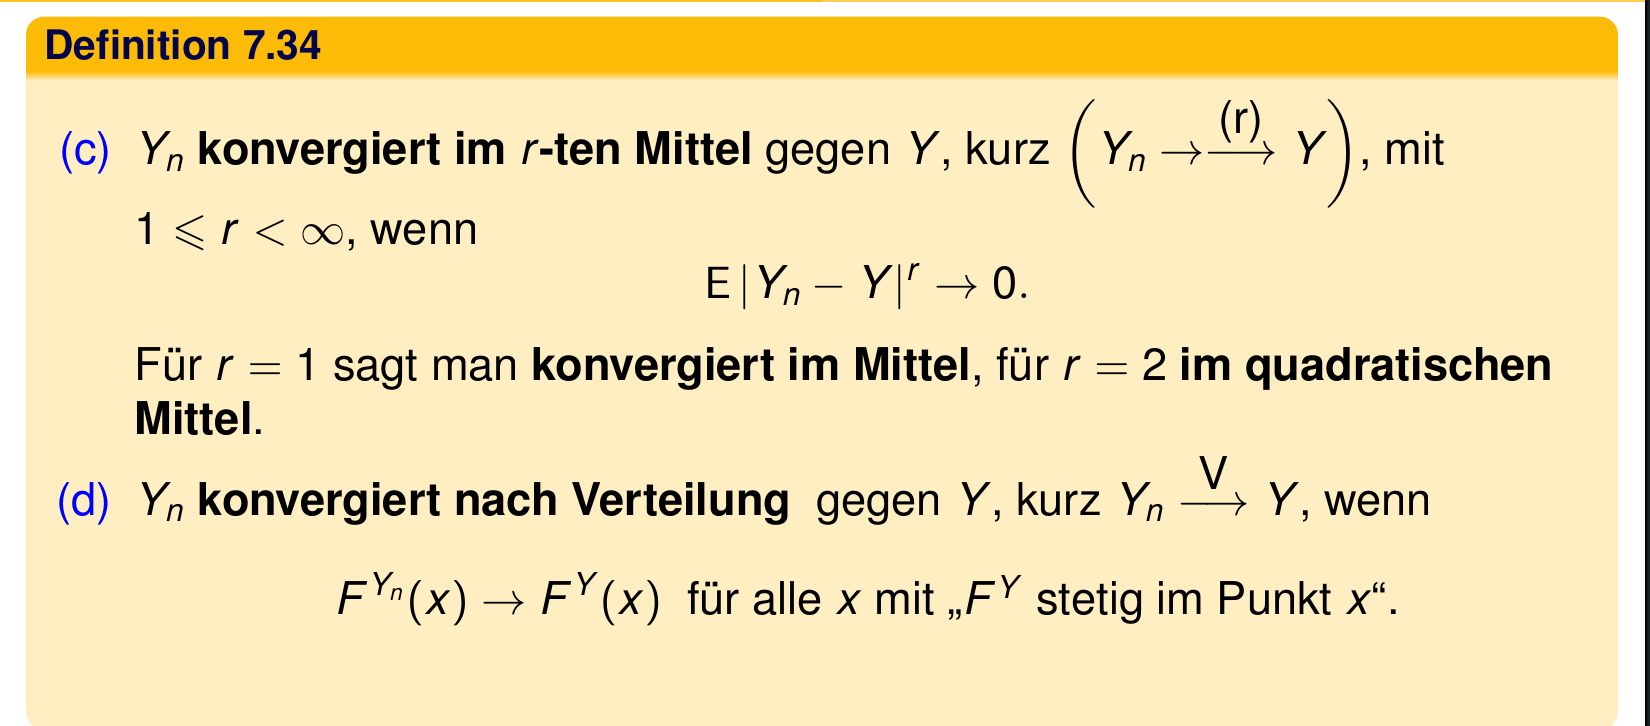
\includegraphics[width=256px]{KonvImErstenMittel.png}\\
	sprich die Mittel konvergieren bzw die Verteilungsfunktion konvergiert für alle stetigen punkte.\\
	\[Z=\frac{X-\mu}{\sigma}\]
	\[EZ=E(\frac{X-\mu}{\sigma}) = \frac{1}{\sigma^2} (EX-\mu)=0\]
	\[EZ=E(\frac{X-\mu}{\sigma}) = \frac{1}{\sigma^2} (EX-\mu)=0\]
	\[\operatorname{Var}(Z)= \operatorname{Var}\left(\frac{X-\mu}{\sigma}\right)=\operatorname{Var}\left(\frac{X}{\sigma}\right) =\frac{1}{\sigma^2} \operatorname{Var}(X) = 1\]


\end{document}

